In the previous chapters, we have outlaid a basic extrapolation framework for ground-state energy sequences coming from NCSM calculations. The network extrapolations have provided suboptimal results for fast converging sequences from \n{3}{H} and \n{4}{He}, as the network consistently predicted a ground-state energy that is too low, especially for the smaller $N_\mathrm{max}$ values, which are important for later use-cases for nuclei whose NCSM calculations cannot be done to a sufficiently high $N_\mathrm{max}$. For the \n{2}{H} nucleus, the networks have predicted values which were too high, but comparable to classical extrapolations coming from exponential function fits.

In this section, we will modify the training data of our extrapolation framework using two different physically motivated training modes in order to to analyze how the training set affects the evaluation of the three nuclei \n{2}{H}, \n{3}{H} and \n{4}{He}. Those modifications only take place in the training process of our networks, meaning the evaluation process is unaffected by those modifications such that they can be assessed in the same way as our basic training mode. This also means that our extrapolation framework is still free of any sort of preselection of the evaluation sequences to provide a more general extrapolation, which takes every available oscillator frequency into account.
\section{Limitation on the model-space dimension}
In the training, we deliberately use NCSM calculations which are calculated to a sufficiently high $N_\mathrm{max}$, to extract the limit as a prediction target for the networks. In our basic training mode, the sequences further got divided into subsequences of four consecutive $N_\mathrm{max}$ values. The network then got trained to predict the same limit value for all of those subsequences. Since there are very high $N_\mathrm{max}$ values available, the training set of input sequences also contains sequences with almost constant values, as the sequences have already converged enough to the limit value at that model-space dimension. The result is that the network also gets trained on converged sequences, for which there is no extrapolation needed. In \autoref{fig:example_nmax}, we can see an example sequence which will be used in training. It is clear that sequences above $N_\mathrm{max} \approx 26$ are almost converged and thus provide no new insights for the network about how to extrapolate unconverged sequences. Furthermore, those sequences might even prevent the networks from extrapolating unconverged sequences, as the networks could learn to just reproduce the lowest value of the sequence, as is the case for the converged sequences.

In order to conform to the later use cases of the extrapolation of unconverged sequences, we should also focus our training on the extrapolation of those sequences. To achieve this, we want to restrict the input sequences to lower values of $N_\mathrm{max}$. As we can already see in \autoref{fig:example_nmax}, a restriction of subsequences to a maximum $N_\mathrm{max}$ of 24 will lead to the exclusion of the extreme cases of converged sequences and an inclusion of high enough $N_\mathrm{max}$ values to allow for different convergence rates in the training set.
\begin{figure}[H]
  \centering
  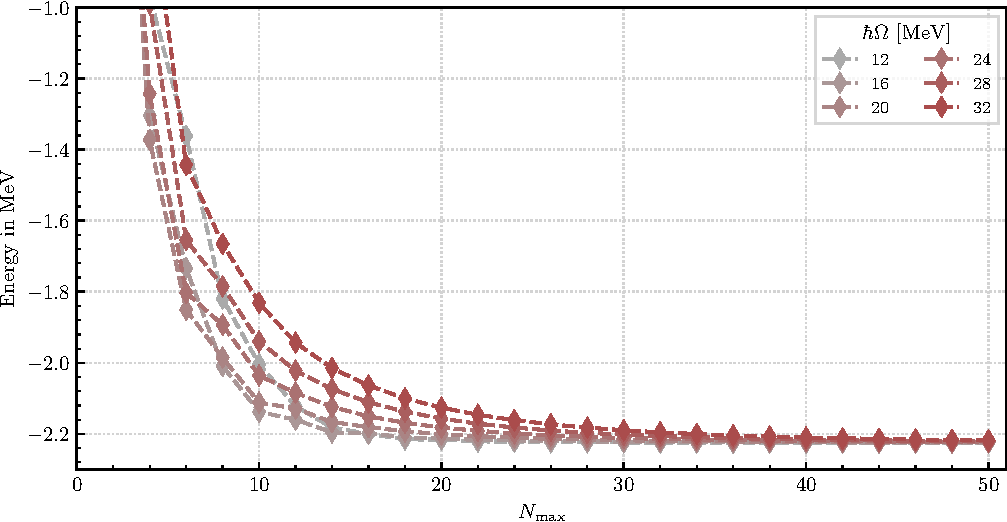
\includegraphics[width=\textwidth]{media/example_sequence.pdf}
  \caption{NCSM results for the $\n{2}{H}$ nucleus. Here, the interaction used for the hamiltonian is \textit{chi2bM3A}. Furthermore, the hamiltionian is SRG evolved using a flow parameter of $\SI{0.04}{\femto\metre^4}$. Each point is the result of a NCSM calculation with a given $N_\mathrm{max}$ and oscillator frequency $\hbar \Omega$.}
  \label{fig:example_nmax}
\end{figure}

\section{Restriction to SRG evolved interactions}
In our second training mode, we want to take another approach to our extrapolation framework as the $N_\mathrm{max}$ limitation training mode. As we have already seen, a SRG evolution of the Hamiltonian results in a faster convergence of the NCSM sequences. Taking this into account, we can also try to train the networks only using NCSM calculations with SRG evolved Hamiltonians using a minimum flow parameter of \srg{0.04}. In doing this, we hope to achieve a more uniform and stronger convergence in the different sequences in the training, such that the networks do not have to extrapolate as much as with unconverged sequences. This will also be useful for the later uses of the extrapolation on heavier nuclei, as an SRG evolution can always be done.

\section{Results and Comparison}
In order to evaluate the training-modified versions of our extrapolation framework, we have to make sure that the evaluation data conforms to the restrictions that we apply to our training set to ensure consistency. In our first training mode, the used $N_\mathrm{max}$ are restricted to be lower than 24. In the second training mode, only interactions which are SRG evolved using a flow parameter of at least \srg{0.04} are used. Our evaluation set, consisting of $N_\mathrm{max}$ values up to 12 and of interactions evolved using a flow parameter of \srg{0.04} and \srg{0.08}, already satisfies these requirement.
\begin{figure}[H]
  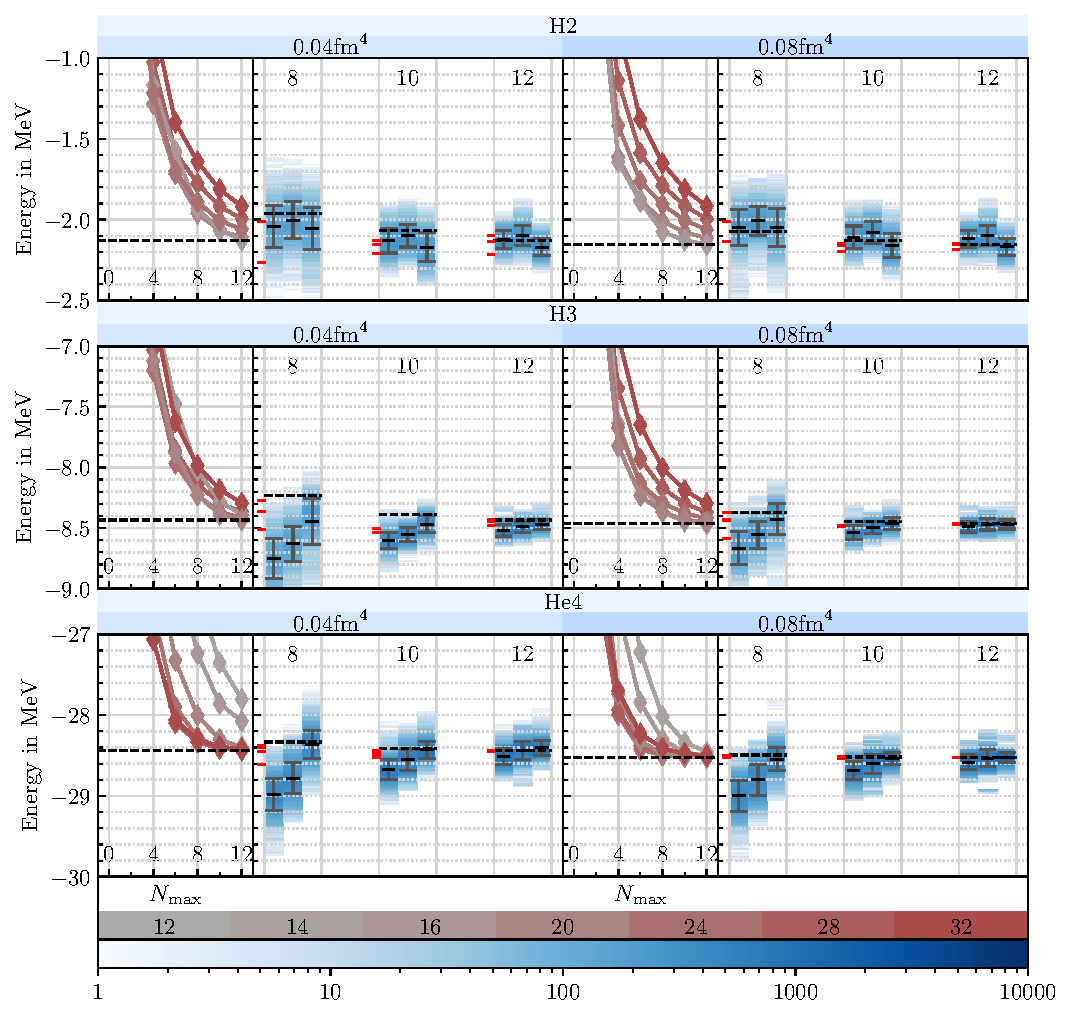
\includegraphics[width=\textwidth]{media/extended_evaluation_ohne_fehlfit.pdf}
  \caption{Evaluation of our training modes on the nuclei \n{2}{H}, \n{3}{H} and \n{4}{He}, using a semi-local momentum space regulated N$^2$LO interaction with two-body interactions and a cutoff at \SI{450}{\mega\electronvolt} \cite{smsquelle}. The shown training modes are, in order from left to right, the basic training mode for comparison, the $N_\mathrm{max}$-limitation training mode and the SRG-filter training mode. For each nucleus and each flow parameter, the NCSM sequences are shown on the left (the different frequencies are colored respectively to the legend, which shows the frequencies $\hbar\Omega$ in \si[]{\mega\electronvolt}) and the extrapolations for a given maximum $N_\mathrm{max}$ on the right. For each maximum $N_\mathrm{max}$, the variational boundary is shown as a dashed line, and the classical extrapolations are shown as red ticks.}
  \label{fig:eval_extended}
\end{figure}

\autoref{fig:eval_extended} displays the evaluation of the three nuclei. Each histogram at every $N_\mathrm{max}$ is now divided into three seperate histograms, showcasing the evaluation result for the different training modes. In each stack of histograms, the leftmost is the basic training mode already introduced in \autoref{chap:framework} and assessed in \autoref{chap:reproduction}. The histogram in the center corresponds to our first training mode, which restricts the $N_\mathrm{max}$ in the training process to at most 24. The rightmost histogram is our second introduced training mode, which restricts the type of training interactions to SRG evolved interactions with a flow parameter of at least \srg{0.04}.

We again begin by looking at the nuclei \n{3}{H} and \n{4}{He}. For both training modes, we see that the predictions get closer to the variational boundary, which means that the training modes yield overall better predictions, since the sequences are already converged enough. Interestingly, the two training modes seem to only impact the accuracy of the prediction. The uncertainty of both training modes are comparable to the uncertainty of the prediction by the basic extrapolation framework.

If we compare the two training modes for those nuclei, we see that the $N_\mathrm{max}$-limitation mode is less impactful than the SRG-filter mode. This can be explained by the fact that the some of the sequences of the \n{3}{H} and the \n{4}{He} nucleus are already converged enough. Since we explicitly remove bare Hamiltonians in the SRG-filter mode, the training set gets limited to a smaller size of fast converging sequences, thus training the net better to those cases. This can especially be seen in the \n{4}{He} nucleus, where there are sequences which have a very strong convergence rate. Here, the SRG-filter mode results lie very close to the variational boundary. The limitation on the $N_\mathrm{max}$ values also have a positive impact on the evaluation. This may indicate that the networks have learned from the constant sequences of high $N_\mathrm{max}$ values to linearly extrapolate the results up to a certain point, which results in the predictions being unreasonably low for low $N_\mathrm{max}$ sequences, as is the case for our basic extrapolation framework.
% 3h, 4he:
% nmax: a bit better
% srg: way better

For the nucleus \n{2}{H}, our basic framework showed a totally different systematic behavior than for the nuclei \n{3}{H} and \n{4}{He}. This is also the case for both new training modes. Especially the $N_\mathrm{max}$ training mode seems to extrapolate not far enough, such that the predictions do not conform to the variational boundary at $N_\mathrm{max} = 12$. Even though the $N_\mathrm{max}$-limitation mode is thought to handle unconverged sequences better than the unmodified training mode, it predicts higher ground-state energies for both SRG flow parameters and for all $N_\mathrm{max}$ values. This can be explained by the fact that the \n{2}{H} sequences are not only converged until $N_\mathrm{max} = 12$, but also converge quite slowly. This leads to a very broad range of energy values at $N_\mathrm{max} = 12$ for all the frequencies, but the sequences themself are relatively flat, leading to a higher prediction of the $N_\mathrm{max}$-limitation training mode. The SRG-filter training mode seems to perform better than the basic training mode. Even though this training mode still produces unreasonably high predictions for $N_\mathrm{max} = 8$, the predictions for all $N_\mathrm{max} \geq 10$ are lower than the variational boundary at $N_\mathrm{max} = 12$. This is a great improvement over the other two training modes.

The comparison between the two different SRG flow parameters yield the same results as in the previous chapter, where we have considered our training without further modifications. We can see that the network predictions do not change much when evaluating the higher srg flow parameter. This is especially interesting in the case of \n{4}{He}, where the difference between the NCSM sequences is the biggest. At $\alpha = \srg{0.04}$, the lower sequences of $\hbar \Omega = \SI{12}{\mega\electronvolt}$ and \SI{14}{\mega\electronvolt} are converging fast, but they have not reached a sufficient degree of convergence, such that the values at $N_\mathrm{max} = 12$ are still spread far apart. For $\alpha = \srg{0.08}$, those sequences have converged sufficiently until $N_\mathrm{max} = 12$. We can see that the networks react very consistently between the different sequences.
% 2h:
% nmax worse than vanilla (WHY?)
% nmax geq 10: srg under varbound!

% difference srg
% same as vanilla: extrapolations go up



\section{Conclusion}
In this chapter, we have extended our basic extrapolation framework by modifying the training process of the neural networks in two distinct ways to see how they affect the extrapolation of ground-state energies. In a first modification, we have decided on only training the networks by using sequences up to $N_\mathrm{max} = 24$. In a second modification, the networks were only trained by NCSM sequences coming from SRG evolved Hamiltionians with a flow parameter $\alpha$ of \srg{0.04} or higher. We have discussed these \textit{training modes} by evaluating the nuclei \n{2}{H}, \n{3}{H} and \n{4}{He} and comparing the results to our basic training mode from \autoref{chap:reproduction}.

To classify our training modes, we first provide two important aspects that those training modes have to show. Firstly, they should result in extrapolations which are "better" in some way when compared to the unmodified training process. For example, they should either result in a smaller uncertainty or in a different prediction which is more reasonable given the NCSM sequences. Secondly, a modification of the training set should result in consistent extrapolations across different scenarios, such as unconverged NCSM sequences and NCSM sequences with a low convergence rate.

Keeping these conditions in mind, we conclude that the SRG-filter training mode so far provided the most reasonable results across all nuclei. The unmodified training mode, as well as the $N_\mathrm{max}$-limitation training mode, predicted unreasonably low ground-state energies for the nuclei \n{3}{H} and \n{4}{He} yet unreasonably high energies for \n{2}{H}. For all of these nuclei, the SRG-filter training mode provided more reasonable predictions. Also, the SRG-filter training mode provided the most consistent results, since it can handle the more converged and more unconverged sequences of \n{3}{H} and \n{4}{He} respectively, as well as the slow converging sequences of \n{2}{H}.

The $N_\mathrm{max}$-limitation filter provided more reasonable results for \n{3}{H} and \n{4}{He}, but too high values for \n{2}{H}, even higher than the unmodified training mode, making it the most unconsistent and unreasonable among the two training modes discussed.

Considering all of the above, it seems that the SRG-filter training mode provides the most promising results. In order to reach a final verdict about the two training modes, we will test how they behave in a scenario which is closer to a real use-case of an extrapolation in \autoref{chap:li6}, where we evaluate the NCSM calculations for the nucleus \n{6}{Li}.
% CONCLUSION
% srg can handle converged and unconverged sequences can be seen by h2 and he4
% Nmax cant handle slow converging sequences

